%! TEX program = LuaTeX

\documentclass[nobackground,dvipsnames,table]{beamer}
\usepackage{cs152}

\mode<presentation>
{\usetheme{Hannover}
    \usecolortheme{cs152}
    \setbeamercovered{transparent}
    \useinnertheme[shadow=false]{rounded}
    \usebackgroundtemplate{}
    \setbeamercolor*{frametitle}{parent=palette primary}
    \setbeamerfont{block title}{size={}}
    \setbeamertemplate{navigation symbols}{}
}

\title{Spam and Fraud}
\subtitle{CS 152 - Trust and Safety Engineering}

\author[A. Stamos]{Alex Stamos}
\institute[SIO]{\large Stanford Internet Observatory}
\date[2022]{\today}
\subject{CS 152 - Trust and Safety Engineering}
\titlegraphic{
\includegraphics[width=5cm]{img/internet-observatory}}

% Change the level of bulleting on the ToC page
\setcounter{tocdepth}{2}

\graphicspath{{img/lesson04}}

\begin{document}

\coverpage

\begin{frame}
    \titlepage
\end{frame}

\begin{frame}{Military Romance Scams}
    \begin{figure}
        \centering
        
\includegraphics[height=0.85\textheight]{military-romance-scam}
    \end{figure}
\end{frame}

\begin{frame}{Nelly Agbogu}
    \begin{figure}
        \centering
        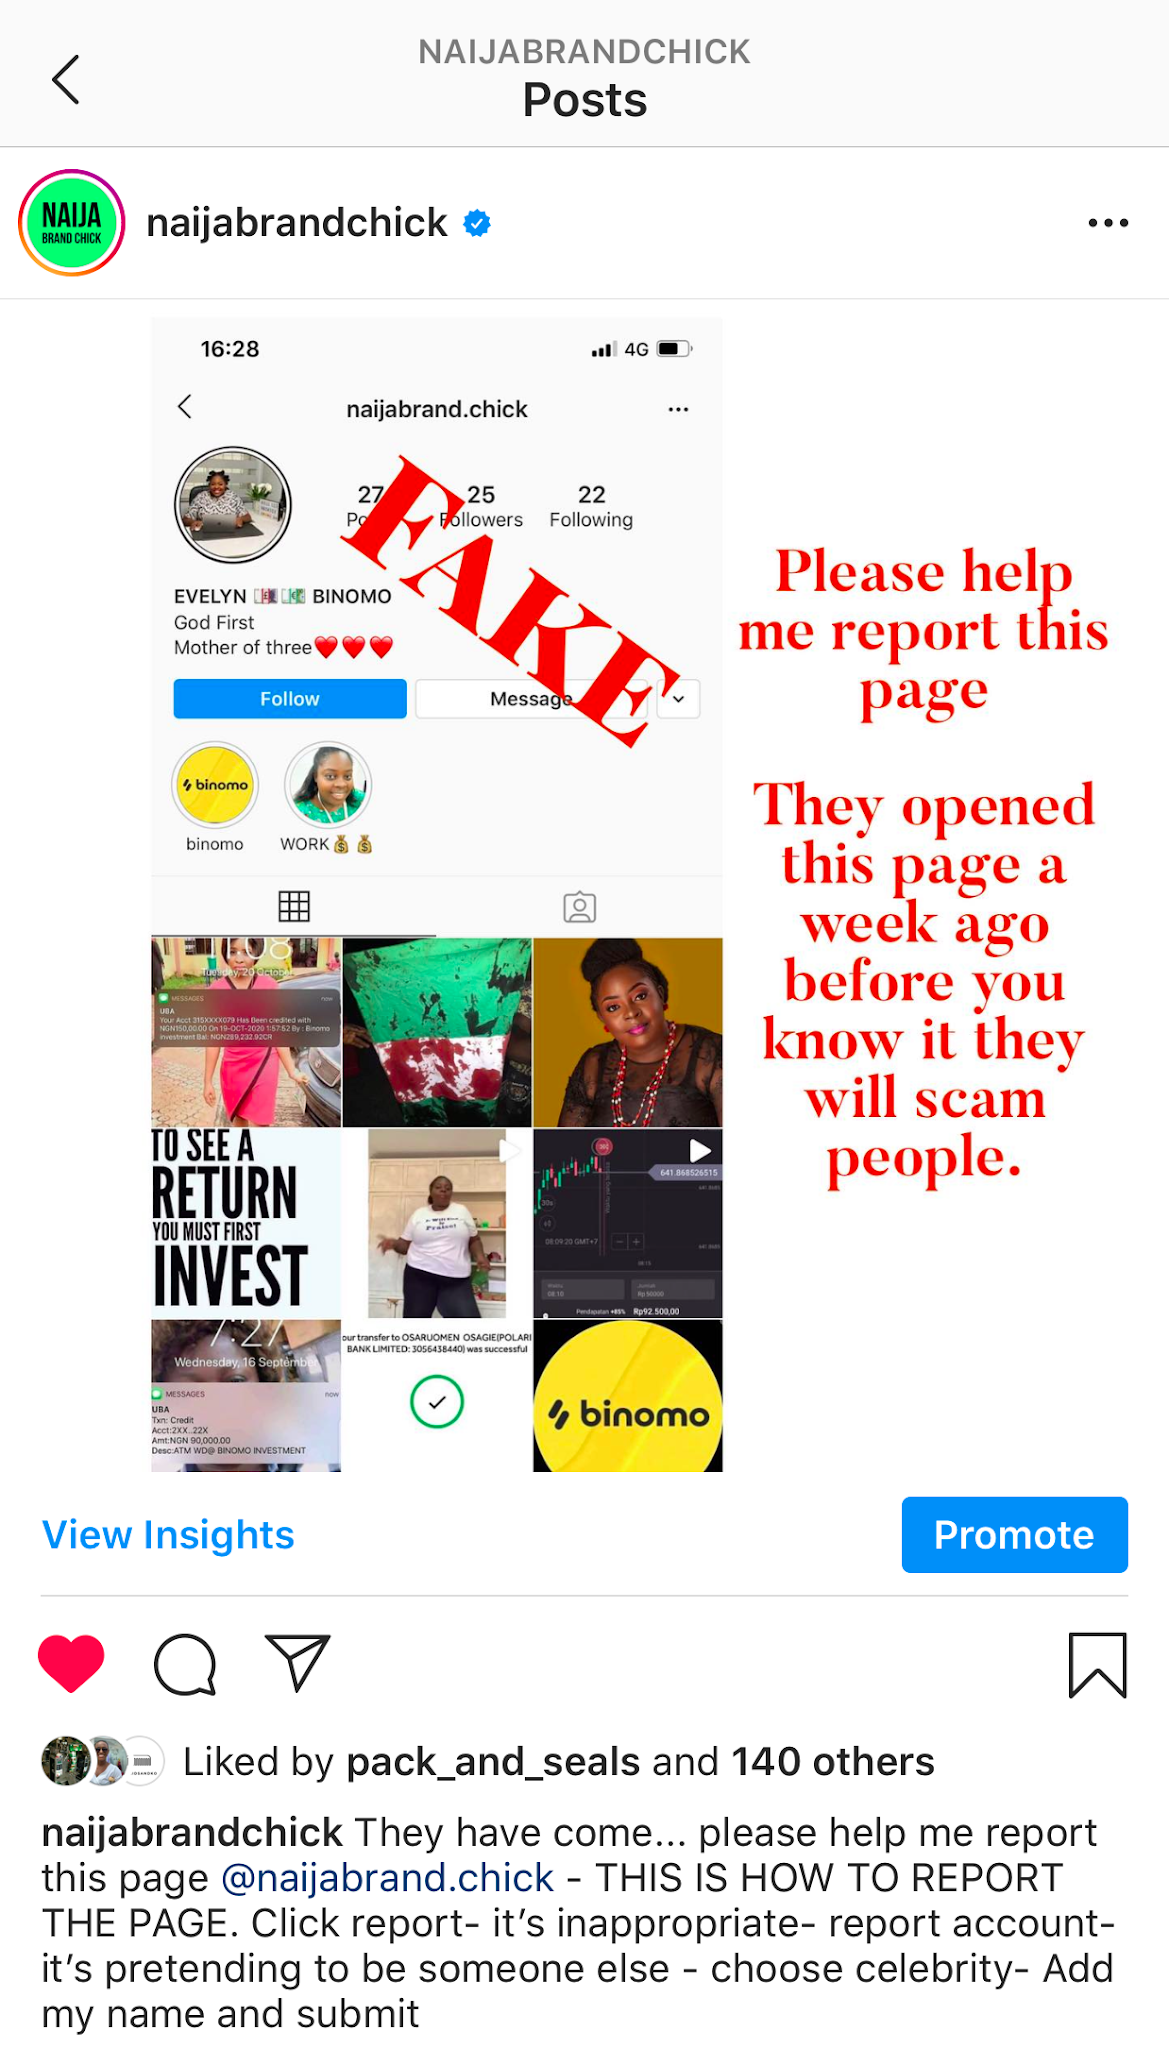
\includegraphics[height=0.85\textheight]{nelly-agbogu}
    \end{figure}
\end{frame}

\begin{frame}{What Will You Learn Today?}
    An overview of the spam ecosystem\\
    An overview of fraud types\\
    A basic understanding of how email works and how it is broken\\
    Some of the basic techniques for spam fighting
\end{frame}

\begin{frame}{}%TODO3 Spam Spam Spam gif - need animate package(?)
    \thispagestyle{empty}
\end{frame}

\section{What is Spam?}

\begin{frame}{What is Spam?}
    \scriptsize
    \begin{columns}[T]
        \column{0.6\textwidth}
            \textbf{NIST:} Electronic junk mail or the abuse of the electronic messaging systems to indiscriminately send unsolicited bulk messages\\~\\
            \textbf{Google:} Spam includes, but is not limited to, unwanted promotional, commercial, or manipulative content that adds little value for users or to Google\\~\\
            \textbf{Facebook:} Content that is designed to deceive, or that attempts to mislead users to increase viewership\\~\\
            \textbf{Reddit:} Repeated, unwanted, and/or unsolicited actions, whether automated or manual, that negatively affect Reddit users, Reddit communities, and/or Reddit itself.
        \column{0.4\textwidth}
            \textbf{TikTok:} Content or activity that seeks to artificially inflate popularity on the platform or attempts to manipulate platform mechanisms to increase interaction metrics.\\~\\
            \textbf{WhatsApp:} Messages that spread false information and are designed to deceive you and prompt you to act in a certain way
    \end{columns}
    \begin{figure}
        \centering
        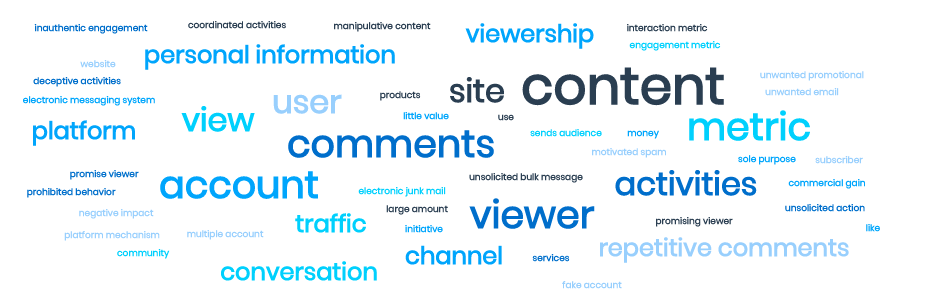
\includegraphics[width=0.75\textwidth]{spam-word-cloud}
    \end{figure}
\end{frame}

\begin{frame}{Primary Purpose of Most Spam}
    \begin{columns}
        \column{0.6\textwidth}
            Deliver information that contains a payload\\
            Payload can be:\\
            \begin{itemize}
                \item Advertising for a product
                \item Bait for a fraud scheme
                \item Phishing site
                \item Computer malware
            \end{itemize}
            %TODO3 google slides figure
        \column{0.4\textwidth}
            \begin{figure}
                \centering
                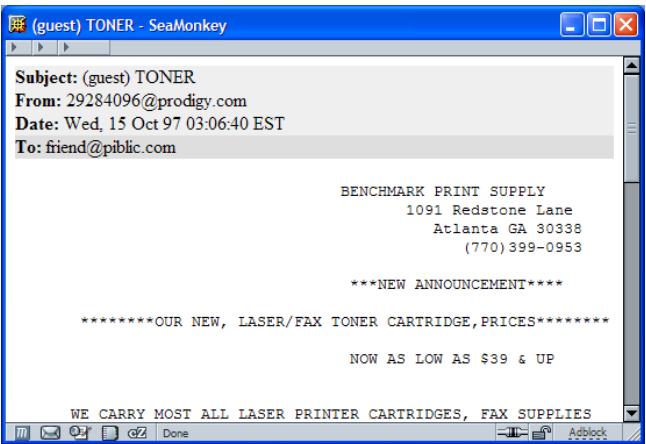
\includegraphics[width=\textwidth]{spam-payload-ad}
                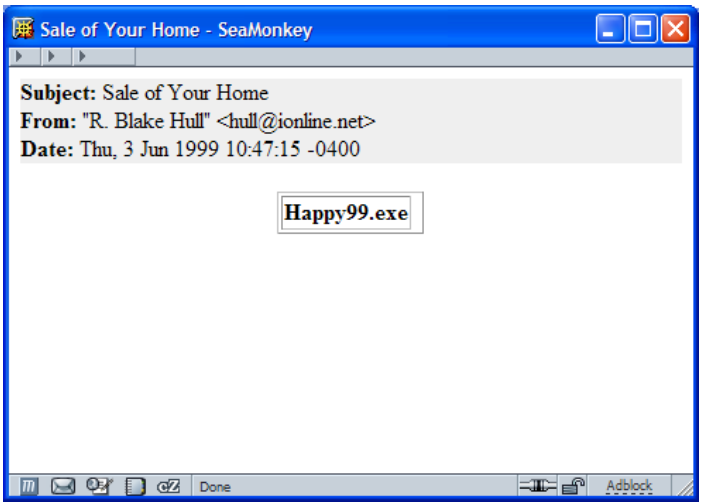
\includegraphics[width=\textwidth]{spam-payload-exe}
            \end{figure}
    \end{columns}
\end{frame}

\begin{frame}{Why Should I Care?}
    \begin{columns}
        \column{0.4\textwidth}
            \begin{itemize}
                \item Spam is the primary vehicle for most cybercrime
                \item Spam is the original trust and safety problem
                \item When any type of abuse can be monetized, the number of people attempting it will explode by orders of magnitude
            \end{itemize}
        \column{0.6\textwidth}
            \begin{figure}
                \centering
                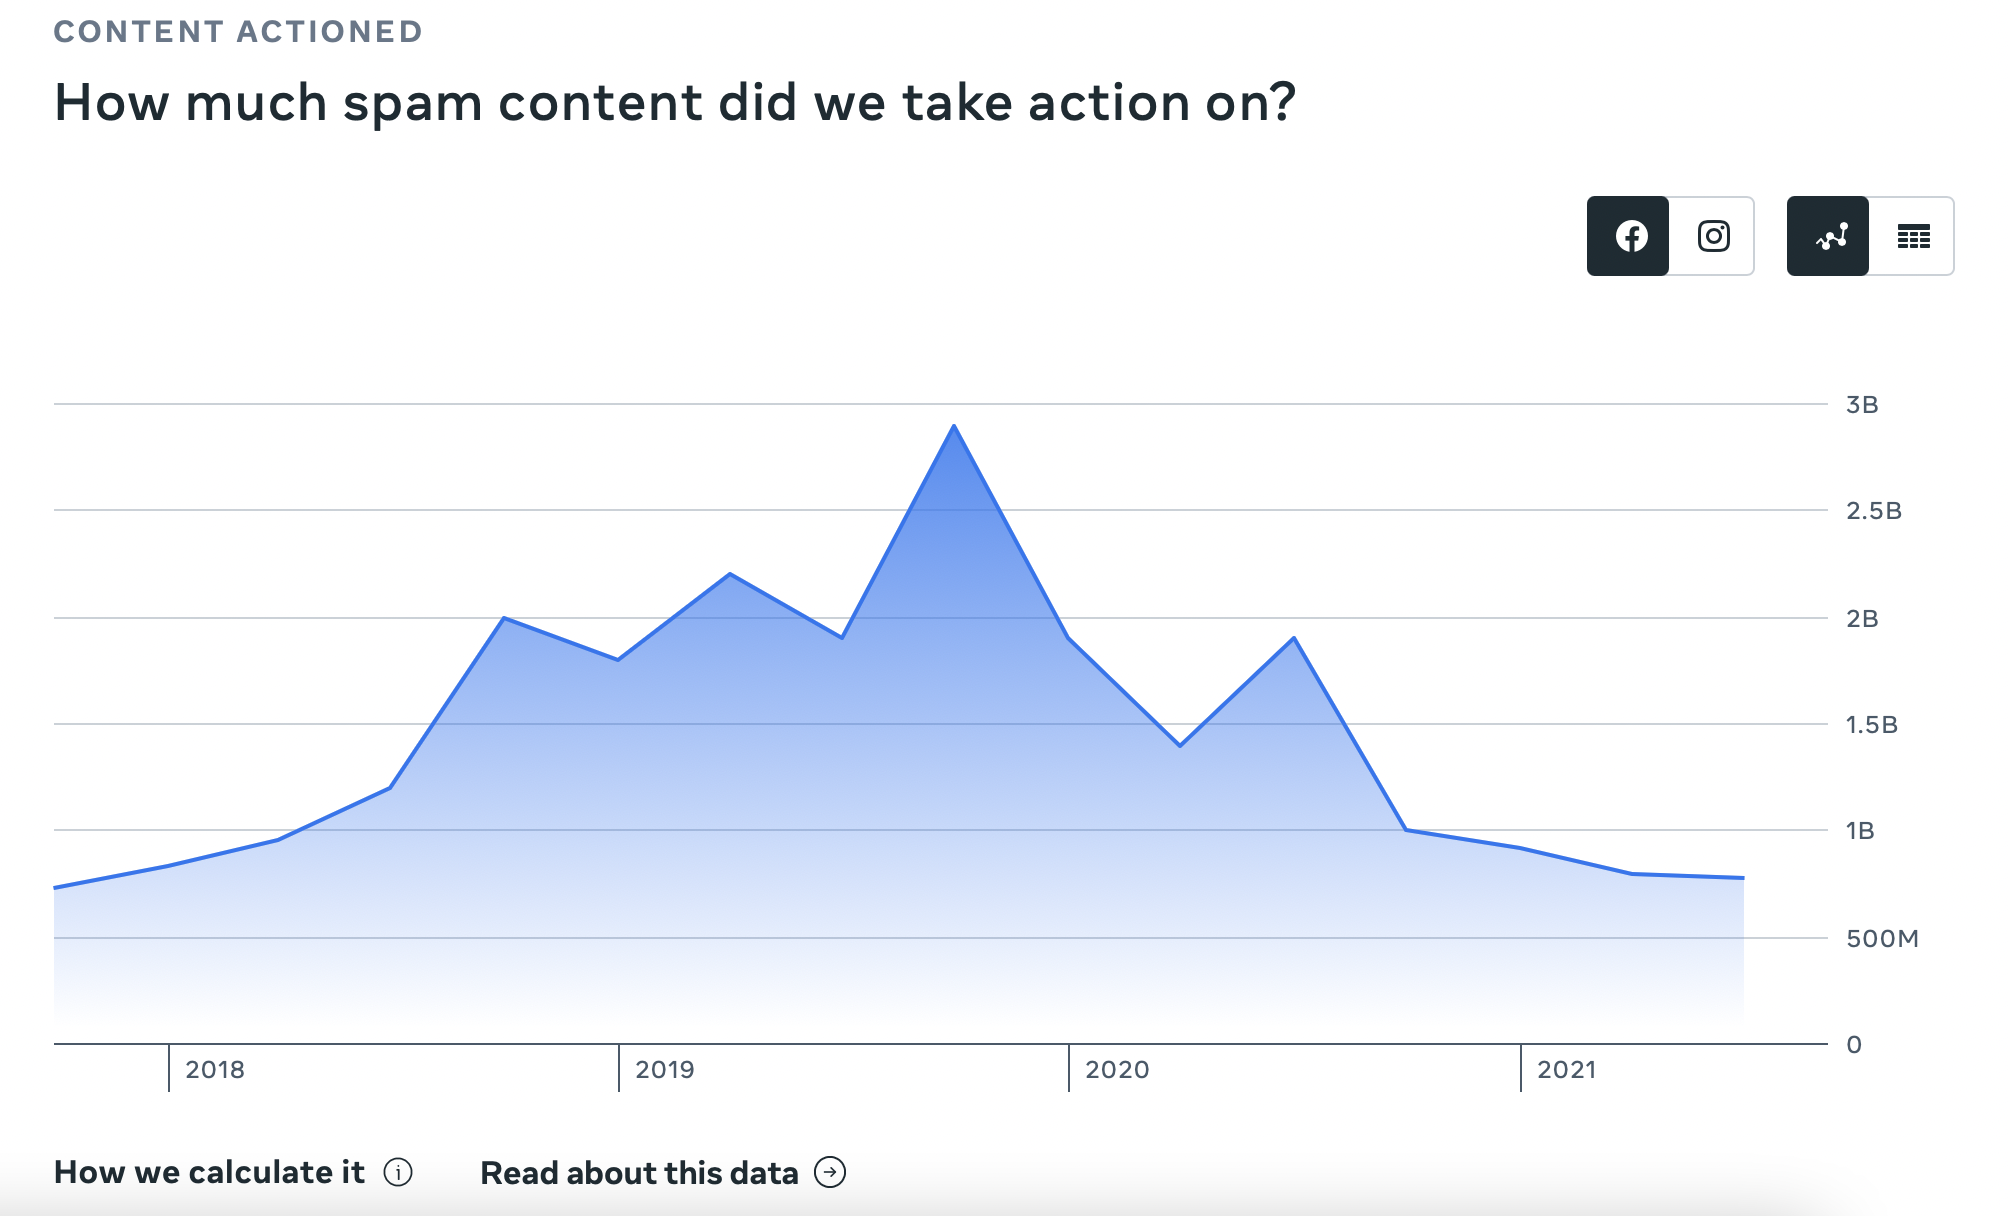
\includegraphics[width=\textwidth]{spam-content-removed}
            \end{figure}
    \end{columns}
\end{frame}

\section{A Brief History of Spam and Fraud}
\begin{frame}{}
    %TODO2 red slide
    A Brief History of Spam and Fraud
\end{frame}

\begin{frame}{History of Spam}
    \scriptsize
    \begin{columns}
        \column{0.7\textwidth}
            Castle-fort of Barcelona\\~\\
            22nd December, 1893\\~\\
            Mr. W. ______\\~\\
            Dear Sir - Notwithstanding having not the pleasure of being acquainted with you, I taken the liberty of writing you this letter in order to trust you with a secret that I never had thought to be obliged to entrust nobody with, but the sufferings that I am enduring in this prison and my love for a young daughter of 16 years old who is in the actuality in a college in Badajoz to make you my revelation, in the hope that you will be good enough as to help me recover a sum of 840,000 pesetas in gold money and french bank-notes that I was one day constrained to hide in the neighbourhood of your locality...\\~\\
            \url{http://www.historyhouse.co.uk/articles/spanish_prisoner_swindle.html}

        \column{0.3\textwidth}
            \begin{figure}
                \centering
                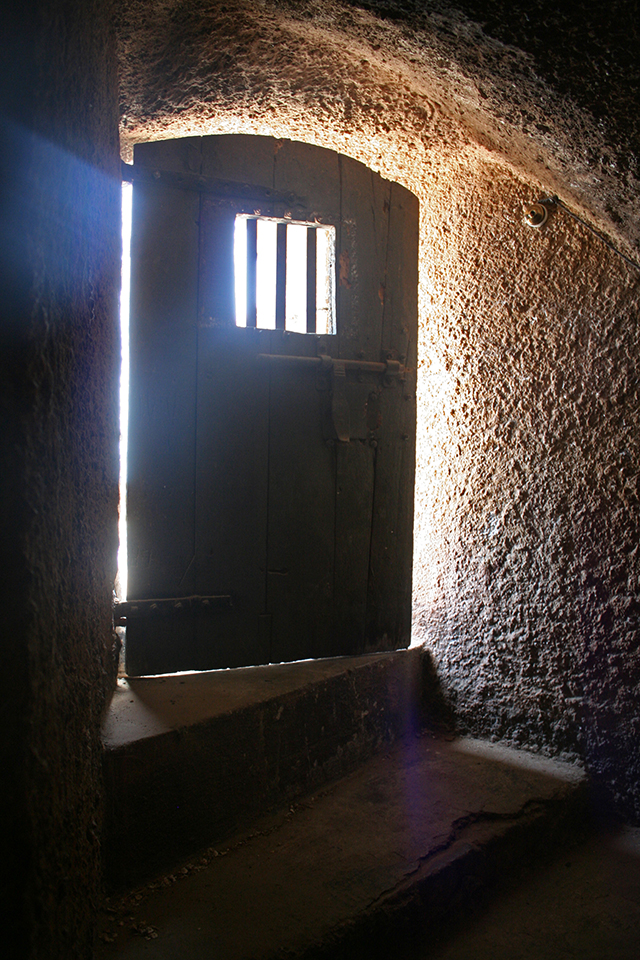
\includegraphics[width=\textwidth]{prison-door}
            \end{figure}
    \end{columns}
\end{frame}

\begin{frame}{2020 Advance Fee Fraud}
    \begin{figure}
        \centering
        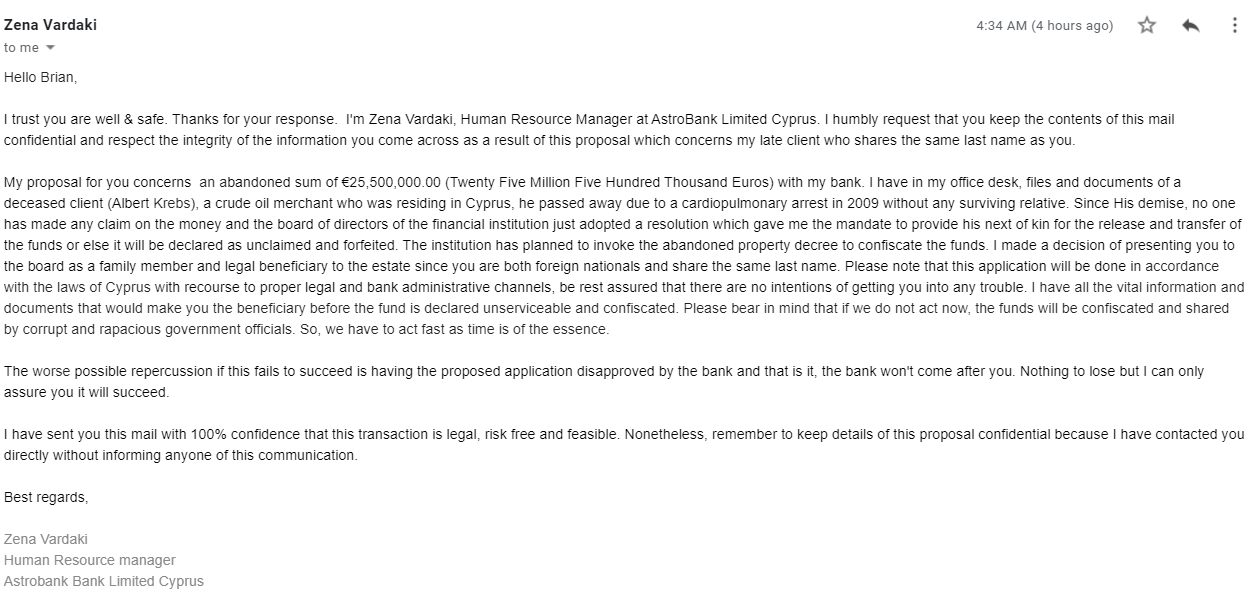
\includegraphics[width=\textwidth]{advance-fee-fraud}
    \end{figure}
    Source: Brian Krebs
\end{frame}

\begin{frame}{History of Spam}
    \begin{itemize}
        \item First commercial spam might be 1978  -- when Digital Equipment Corporation sent advertising mail to ARPAnet email users.
        \item Or it might be 1971 when an MIT computer administrator decided everybody on the computer needed to know “THERE IS NO WAY TO PEACE. PEACE IS THE WAY.”
        \item Or it could be 1864: 
    \end{itemize}
    \begin{columns}
        \column{0.35\textwidth}
            \begin{figure}
                \centering
                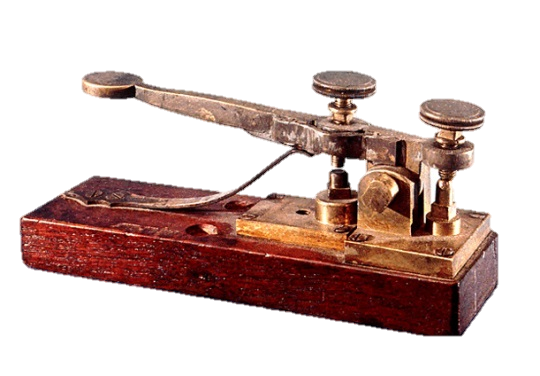
\includegraphics[width=\textwidth]{telegraph}
            \end{figure}
        \column{0.65\textwidth}
            \begin{figure}
                \centering
                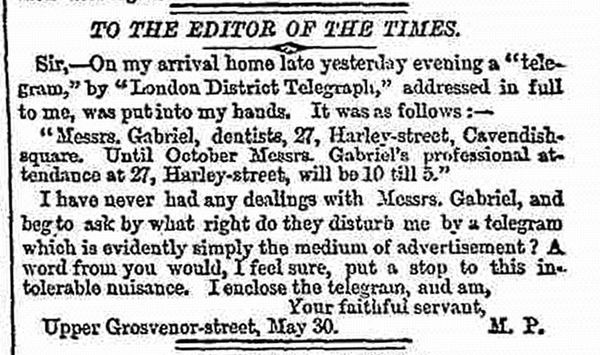
\includegraphics[width=\textwidth]{telegram-spam}
            \end{figure}
    \end{columns}
\end{frame}

\begin{frame}{One Thing That Unifies All The "First" Spams}
    Their senders believe:\\
    \begin{itemize}
        \item That they were doing a good and useful thing
        \item That people who complain are just unkind
    \end{itemize}
    The two chief problems getting rid of spam are:\\
    \begin{enumerate}
        \item Different people have different opinions on what is spam
        \item Advertising is useful and successful 
    \end{enumerate}
\end{frame}

\begin{frame}{Large-Scale Commercial Spam}
    \begin{columns}
        \column{0.5\textwidth}
            Most early spam consisted of messages from pranksters, chain letters, and inappropriate messages\\
            Unsolicited commercial spam was quite rare\\
            Until Canter and Siegel...
        \column{0.5\textwidth}
            \begin{figure}
                \centering
                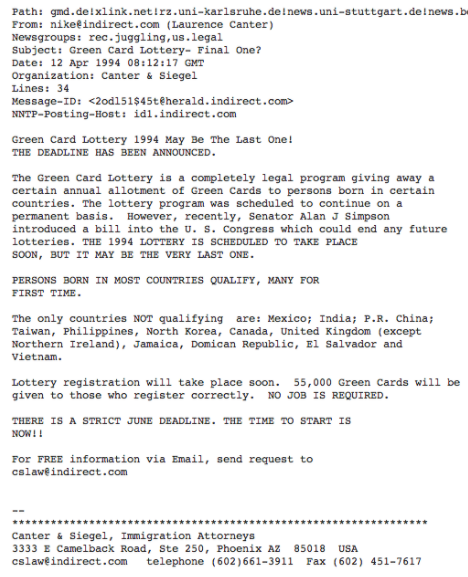
\includegraphics[width=\textwidth]{canter-and-siegel}
            \end{figure}
    \end{columns}
\end{frame}

\begin{frame}{The Growth of Email Spam}
    \begin{columns}
        \column{0.5\textwidth}
            \begin{figure}
                \centering
                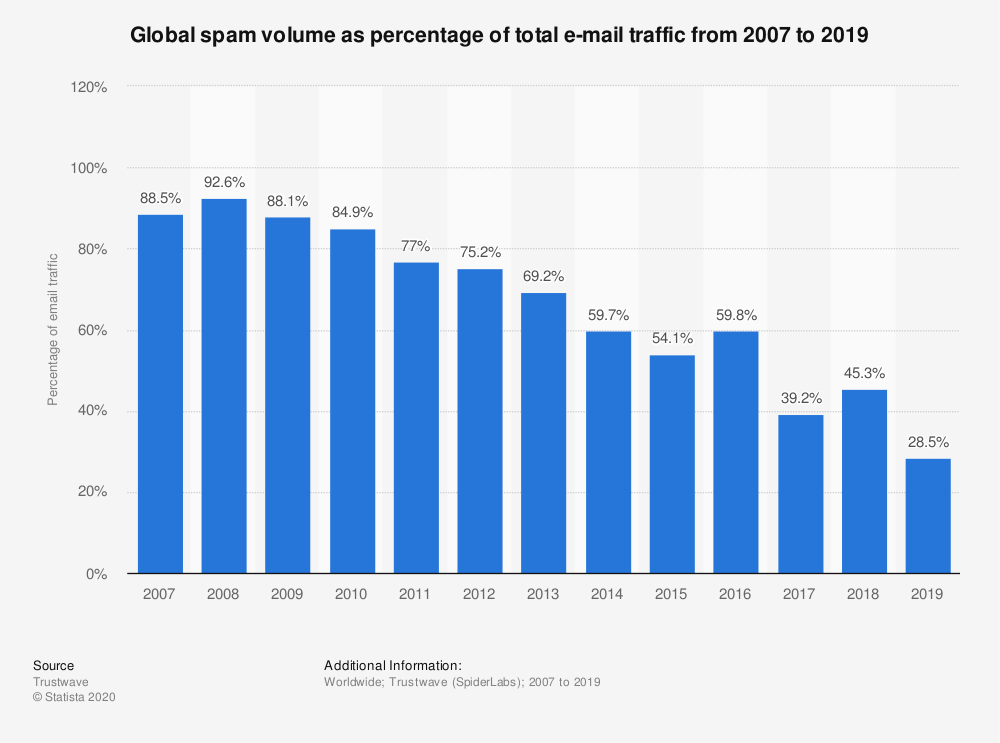
\includegraphics[width=\textwidth]{spam-percent}
            \end{figure}
        \column{0.5\textwidth}
            \begin{itemize}
                \item Spam increased rapidly until it reached as much as 90\% of all mail.
                \begin{itemize}
                    \item Measuring spam is hard because most mail systems reject a lot of mail before finalizing it. \\~\\
                \end{itemize}
                
                \item Many statistics show spam declining from peak
                \begin{itemize}
                    \item Measurement of these kinds of issues is dynamic and based upon a small set of actors
                \end{itemize}
            \end{itemize}
    \end{columns}
\end{frame}

\begin{frame}{Spam as Criminal Enterprise}
    \begin{columns}
        \column{0.4\textwidth}
            \begin{itemize}
                \item Most spam is illegal
                \item Spam is now a specialized industry
                \item Cybercriminals developing more sophisticated tactics to evade anti-spam defenses
                \item Rise of “bulletproof” hosting providers
            \end{itemize}
        \column{0.6\textwidth}
            \begin{figure}
                \centering
                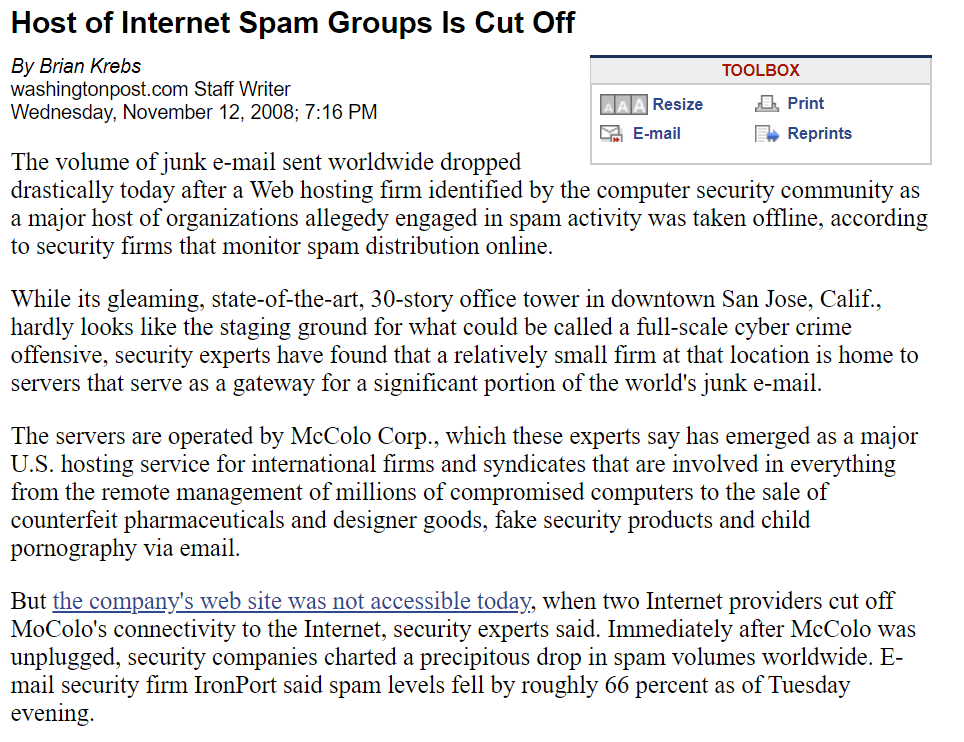
\includegraphics[width=\textwidth]{spam-groups-cut-off}
            \end{figure}
    \end{columns}
\end{frame}

\begin{frame}{The Rise of Botnets}
    \begin{itemize}
        \item First spamming botnets appeared in 2003
        \item Collection of internet-connected computers infected by malware
        \item Controlled through command-and-control servers
        \item Deployed to perform automatic tasks, eg click fraud 
        \item Cost-effective
    \end{itemize}
    \begin{figure}
        \centering
        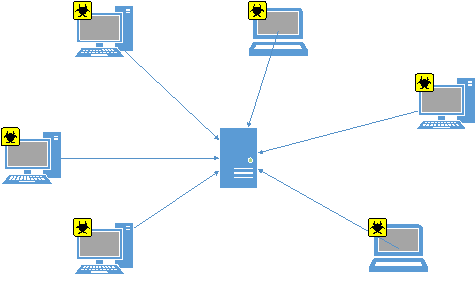
\includegraphics[width=0.5\textwidth]{botnet}
    \end{figure}
\end{frame}

\begin{frame}{Spam is a Well-Developed Ecosystem}
    You can buy
    \begin{itemize}
        \item Software to send spam
        \item Time on other people’s computers to run the software
        \item Lots of ways to monetize the clicks
        \item Addresses to send mail to
        \item Accounts to send mail from
    \end{itemize}
    But you will be buying them from criminals who are not always honest sellers.
    \begin{figure}
        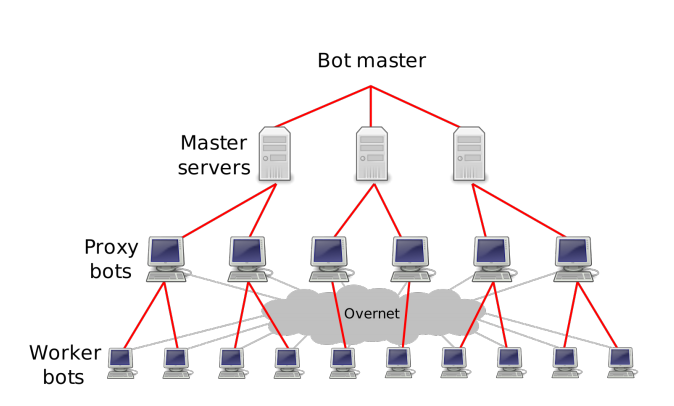
\includegraphics[width=0.5\textwidth, right]{botnet-structure}
    \end{figure}
\end{frame}

\section{What Does Current Spam Look Like?}

\begin{frame}{What Does Current Spam Look Like?}
    \begin{itemize}
        \item Affiliate marketing
        \item Dodgy marketing
        \item Fraud
        \item Web spam
        \item Social spam
    \end{itemize}
\end{frame}

\begin{frame}{Fraud}
    \begin{columns}
        \column{0.6\textwidth}
            Intentionally and knowingly deceiving a victim by misrepresenting, concealing or omitting facts about promised goods, services, or other benefits for monetary gain
        \column{0.4\textwidth}
            \begin{figure}
                \centering
                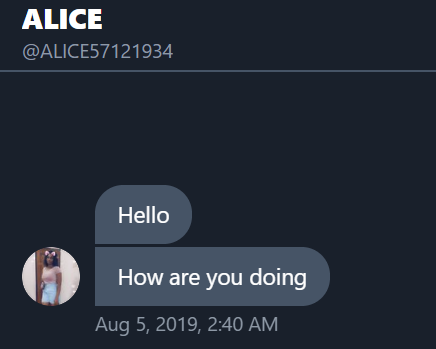
\includegraphics[width=\textwidth]{ALICE}
            \end{figure}
    \end{columns}
    Common internet fraud schemes include:
    \begin{columns}
        \column{0.5\textwidth}
            \begin{itemize}
                \item Romance fraud
                \item Advance fee fraud
                \item Shopping fraud
                \item Payment and physical goods fraud
            \end{itemize}
        \column{0.5\textwidth}
            \begin{itemize}
                \item Extortion and digital kidnapping
                \item Fake antivirus software
                \item Fake charities
                \item Fake lotteries/prizes
                \item Fake debt help
            \end{itemize}
    \end{columns}
\end{frame}

\begin{frame}{}%TODO2 blank slide
    \thispagestyle{empty}
    \footnotesize
    You don’t know me and you’re thinking why you received this email, right?\\
    Well, I actually placed a malware on the porn website and guess what, you visited this web site to have fun (you know what I mean). While you were watching the video, your web browser acted as a RDP (Remote Desktop) and a keylogger which provided me access to your display screen and webcam. Right after that, my software gathered all your contacts from your Messenger, Facebook account, and email account.\\
    What exactly did I do?\\
    I made a split-screen video. First part recorded the video you were viewing (you’ve got a fine taste haha), and next part recorded your webcam (Yep! It’s you doing nasty things!).\\
    What should you do?\\
    Well, I believe, \$1400 is a fair price for our little secret. You’ll make the payment via Bitcoin to the below address (if you don’t know this, search “how to buy bitcoin” in Google).\\
    BTC Address: 1Dvd7Wb72JBTbAcfTrxSJCZZuf4tsT8V72\\
    (It is cAsE sensitive, so copy and paste it)\\
    Important:\\
    You have 24 hours in order to make the payment. (I have an unique pixel within this email message, and right now I know that you have read this email). If I don’t get the payment, I will send your video to all of your contacts including relatives, coworkers, and so forth. Nonetheless, if I do get paid, I will erase the video immidiately. If you want evidence, reply with “Yes!” and I will send your video recording to your 5 friends. This is a non-negotiable offer, so don’t waste my time and yours by replying to this email.
\end{frame}

\begin{frame}{Cryptocurrencies Have Supercharged This Market}
    \begin{figure}
        \centering
        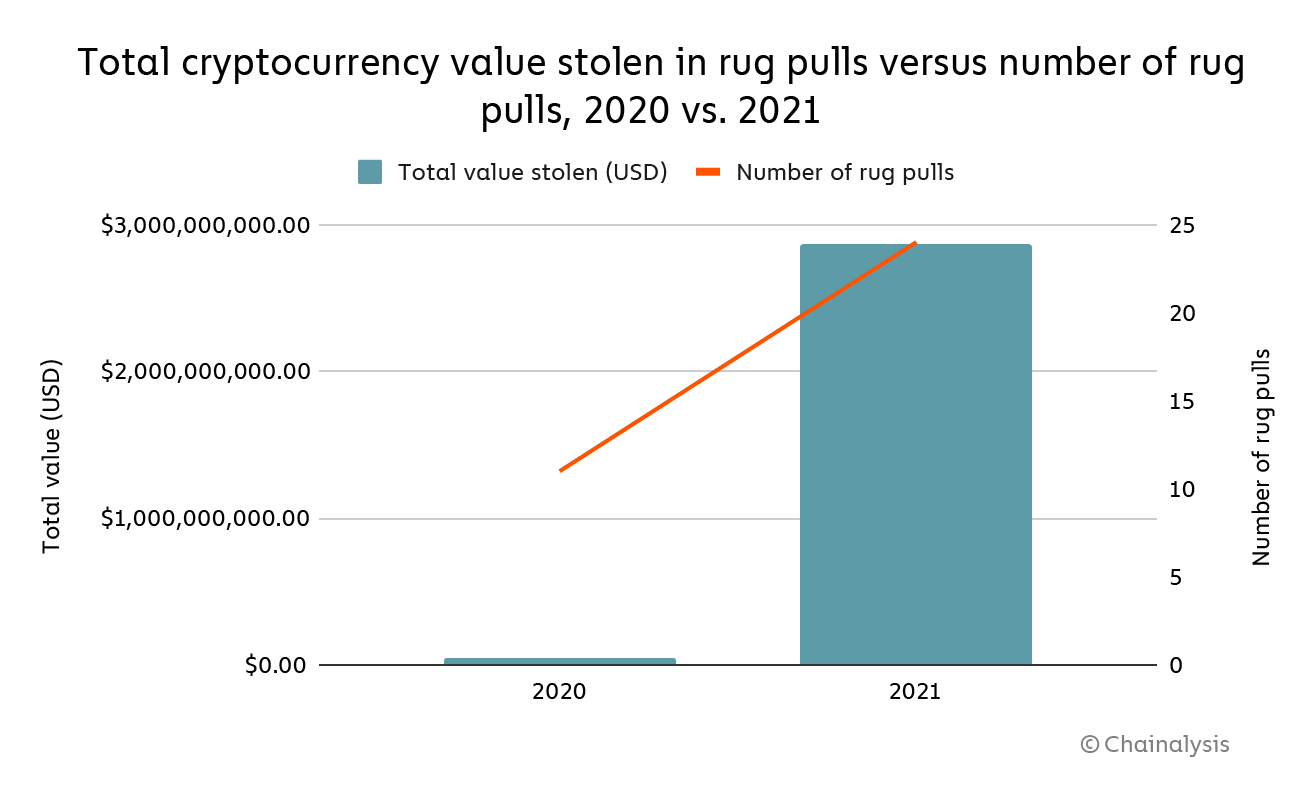
\includegraphics[width=\textwidth]{rug-pulls}
    \end{figure}
    \url{https://blog.chainalysis.com/reports/2021-crypto-scam-revenues/}
\end{frame}

\begin{frame}{Social Spam}
    \begin{columns}
        \column{0.34\textwidth}
            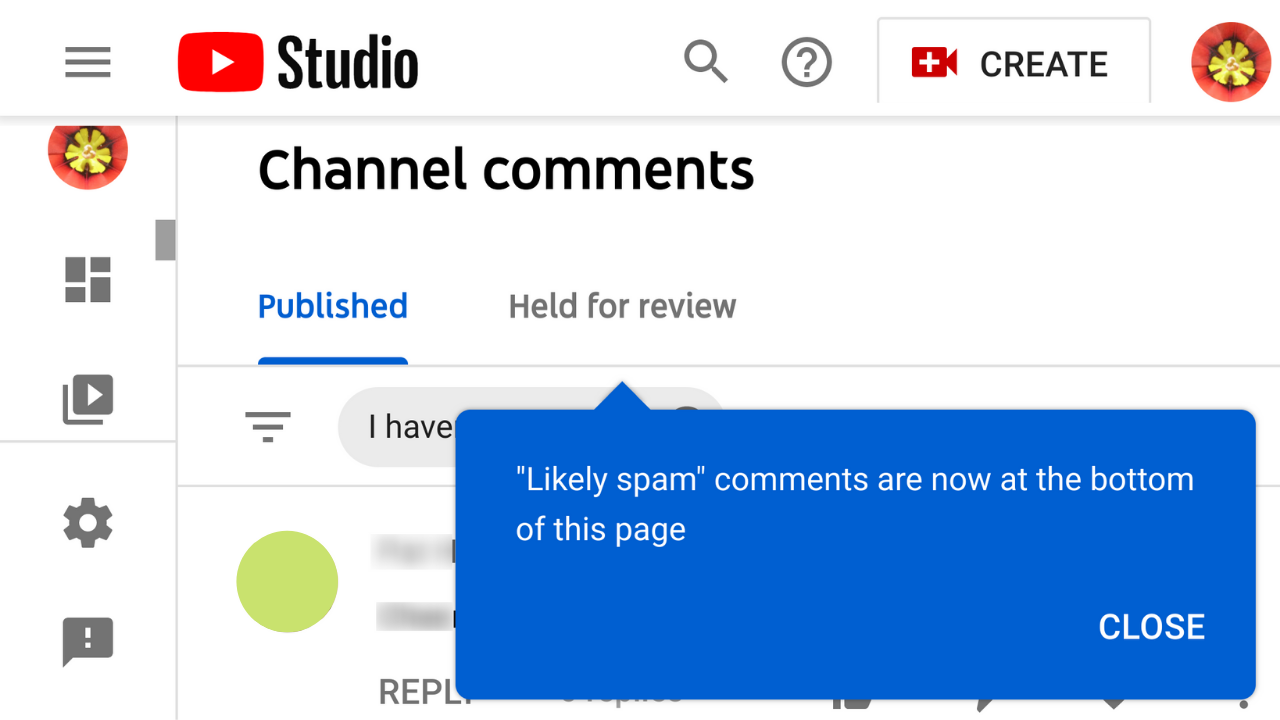
\includegraphics[width=\textwidth]{yt-social-spam}
        \column{0.3\textwidth}
            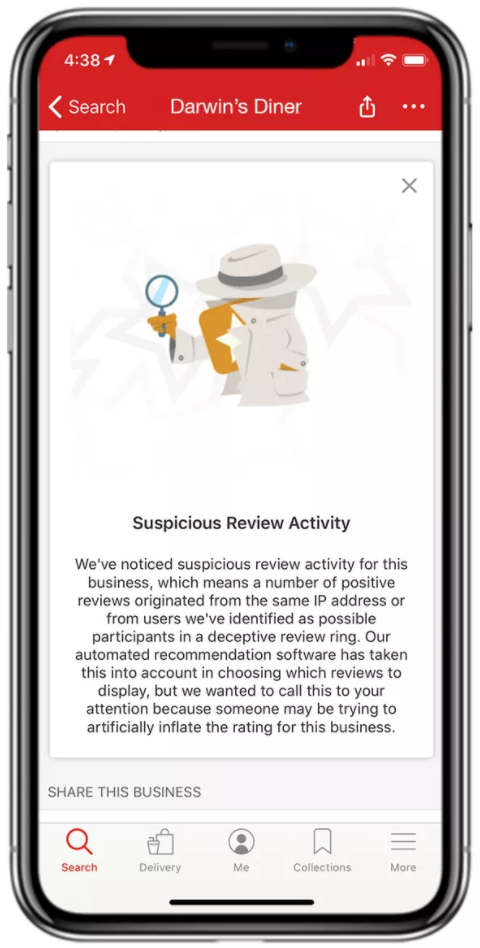
\includegraphics[width=\textwidth]{yelp-spam}
        \column{0.34\textwidth}
            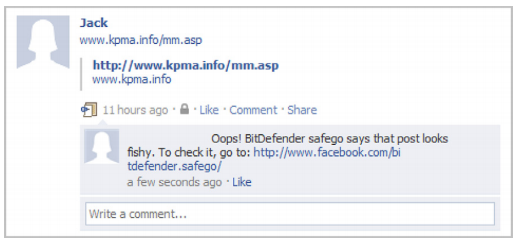
\includegraphics[width=\textwidth]{facebook-spam}
    \end{columns}
\end{frame}

\begin{frame}{Web Spam}
    Trying to get better placement in search results by using various tricks\\~\\
    \begin{columns}
        \column{0.3\textwidth}
            Examples:\\
            Hidden text\\ 
            Doorway pages\\ 
            Cloaking\\
            Sneaky redirects
        \column{0.7\textwidth}
            \begin{figure}
                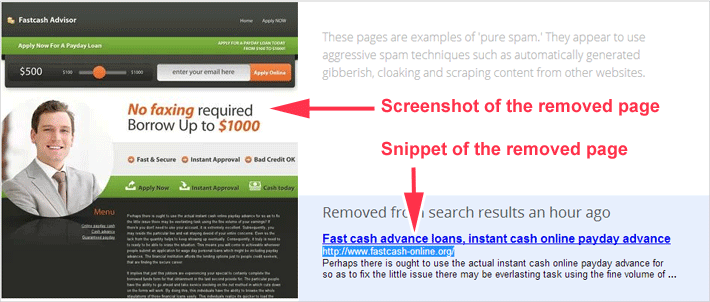
\includegraphics[width=\textwidth, right]{fastcash}
            \end{figure}
    \end{columns}
\end{frame}

\section{Responses and Mitigations}

\begin{frame}{}
    Responses and Mitigations
    %TODO2 red slide
\end{frame}

\begin{frame}{Policy Responses}
    \begin{itemize}
        \item Identify how spammers use your products
        \item Create industry working groups
        \item Create and adopt industry standards, eg Apache SpamAssassin
        \item Enforce identity policies
        \item Reduce low quality links
        \item Seek outside counsel to identify legal responsibilities and offensive options
    \end{itemize}
\end{frame}

\begin{frame}{Product/Technical Responses}
    \begin{itemize}
        \item Utilize machine learning for spam and fake account detection
        \item Implement verification checkmarks
        \item Build out spam reporting mechanisms
        \item Operational checks on well-known targets
        \item Threat Intelligence to stay one step ahead
    \end{itemize}
\end{frame}

\begin{frame}{Aren’t There Easy Fixes to Spam?}
    \begin{itemize}
        \item Block words like “viagra”
        \item Charge money to send email
        \item But I already have a spam filter that does 95\% of a test corpus
        \item Just change how email works entirely
    \end{itemize}
\end{frame}

\begin{frame}{Block Keywords - Example: Viagra}
    \begin{columns}[T]
        \column{0.5\textwidth}
            Cases of wanted use:
            \begin{itemize}
                \item Messages with your doctor
                \item Messages with your intimate partner
                \item Pfizer employees
                \item Messages with your friends 
                \item Directions (“\textbf{via Gra}ves End”)
            \end{itemize}
        \column{0.5\textwidth}
            Cases of unwanted use:
            \begin{itemize}
                \item Unsolicited sales emails
            \end{itemize}
            \begin{figure}
                
\includegraphics[width=0.6\textwidth]{viagra}
            \end{figure}
    \end{columns}\\~\\
    %TODO3 bigger space btwn examples
    \centering
    \textit{\textbf{Can your algorithm catch this?} \\~\\
    v*i*a_g*r*a     vi(@)gr@		V|i|a|g|r|a	  \textbackslash/¡å9®á		viiagra\\~\\
    (there are over $10^{21}$ ways to spell viagra)}
\end{frame}

\begin{frame}{Block Keywords}
    \begin{columns}
        \column{0.3\textwidth}
            \begin{itemize}
                \item Still have problem of  image spam 
                \item Multiple methods to defeat anti-spam filters
            \end{itemize}
            \begin{figure}
                \centering
                
\includegraphics[width=\textwidth]{viagra-ad}
            \end{figure}
        \column{0.7\textwidth}
            \begin{figure}
                \centering
                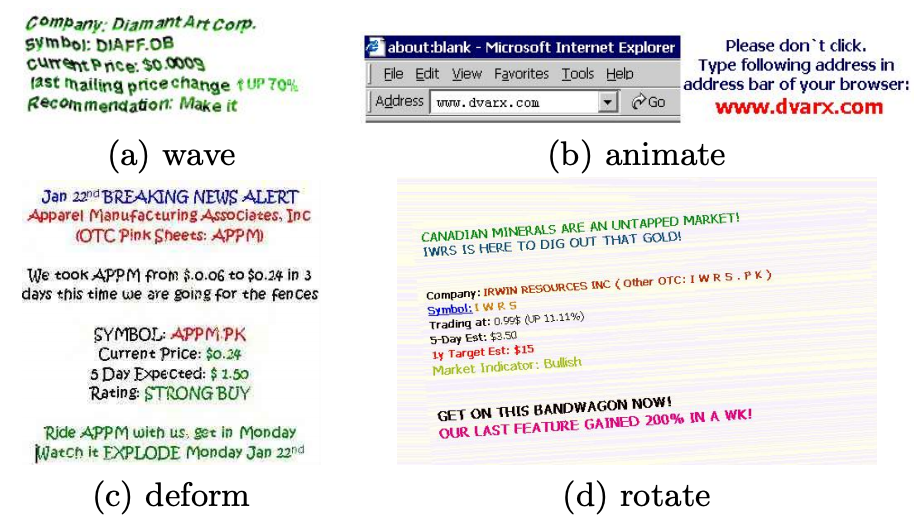
\includegraphics[width=\textwidth]{keyword-blocking-bypass}
            \end{figure}
    \end{columns}
\end{frame}

\begin{frame}{Charge Money for Sending Email}
    %TODO3 table
\end{frame}

\begin{frame}{What About a 95\% Accurate Solution?}
    High volume requires high precision 
    \begin{itemize}
        \item Yahoo averages 30 billion send attempts a day.
        \item Yahoo delivers about 4 billion, including messages that go to the spam folder.
        \item 5\% of 4 billion is 200 million
        \item 5\% of 30 billion is 1.5 billion
    \end{itemize}
    \begin{figure}
        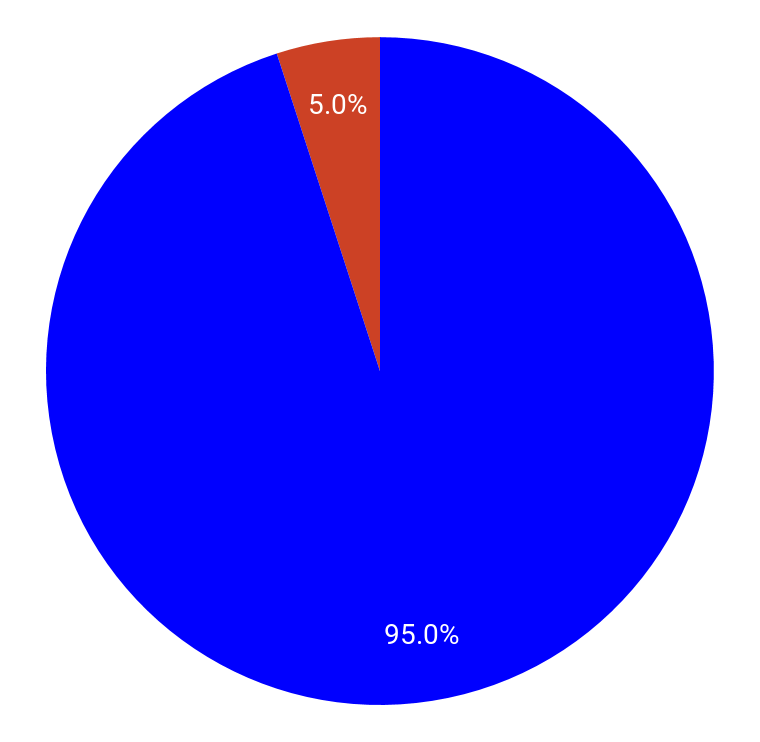
\includegraphics[width=0.25\textwidth]{95-percent}
    \end{figure}
\end{frame}

\begin{frame}{Spam is not a mosquito problem; it’s a squirrel problem}
    %TODO3 birdfeeder gif - need animate package
    (this is a squirrel proof birdfeeder)
\end{frame}

\begin{frame}{Just Change How the Whole Thing Works}
    The primary advantage of email is that it’s a rich and open ecosystem\\
    The slowest moving parts of that ecosystem include important parts
    \begin{itemize}
        \item Governments
        \item Access for people who do not have their own Internet connections
        \item Hardware devices, including adaptive devices for the handicapped
    \end{itemize}
\end{frame}

\section{How Does Email Work?}

\begin{frame}{How Does Email Work? – First, the Players}
    \textbf{MUA = Mail User Agent}
    \begin{itemize}
        \item The thing that shows you your mail
    \end{itemize}
    
    \textbf{MTA = Mail Transfer Agent}
    \begin{itemize}
        \item All the things between you and your recipient
    \end{itemize}
    
    \textbf{MSA = Mail Storage Agent}
    \begin{itemize}
        \item Where your mail is when you're not reading it
    \end{itemize}
\end{frame}

\begin{frame}{How Email Works}
    %TODO3 diagram
\end{frame}

\begin{frame}{What is an RFC?}
    \begin{columns}
        \column{0.5\textwidth}
            \begin{itemize}
                \item (Not really a) Request For Comment
                \item The basic documents of the IETF, the Internet Engineering Task Force
                \item Which is a bunch of volunteers (in theory speaking as individuals) who make up standards for the Internet
            \end{itemize}
            Reality is running code, which sometimes differs significantly from the RFC
        \column{0.5\textwidth}
            \begin{figure}
                \centering
                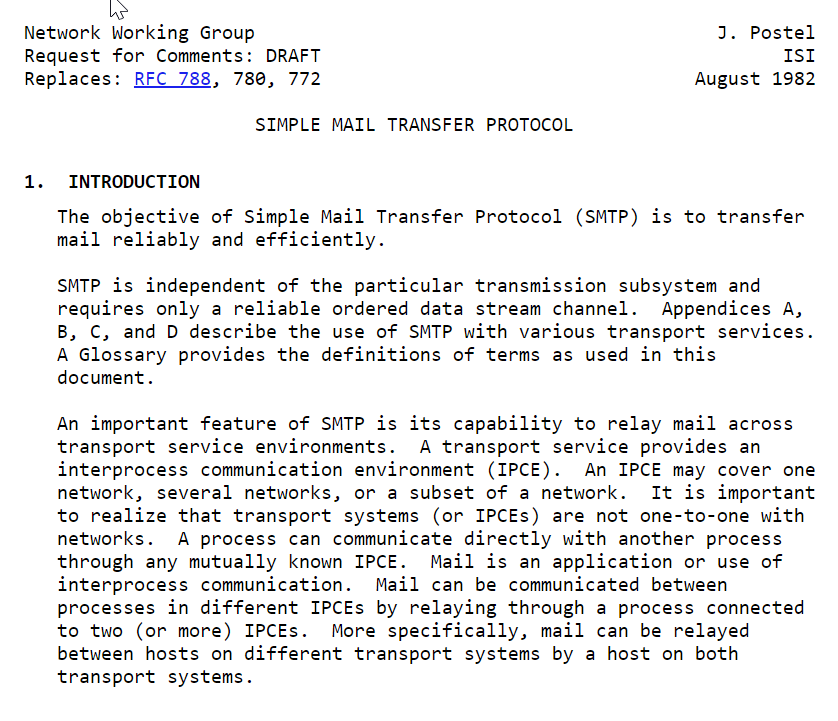
\includegraphics[width=\textwidth]{SMTP}
            \end{figure}
    \end{columns}
\end{frame}

\begin{frame}{Sample SMTP Dialog, Envelope}
    \textcolor{blue}{220 smtp.example.com ESMTP Postfix\\}
    HELO relay.example.org\\
    \textcolor{blue}{250 Hello relay.example.org, I am glad to meet you\\}
    MAIL FROM:<bob@example.org>\\
    \textcolor{blue}{250 Ok\\}
    RCPT TO:<alice@example.com>\\
    \textcolor{blue}{250 Ok\\}
    RCPT TO:<theboss@example.com>\\
    \textcolor{blue}{250 Ok\\}
    DATA\\
    \textcolor{blue}{354 End data with <CR><LF>.<CR><LF>}
\end{frame}

\begin{frame}{Sample SMTP Dialog, Body}
    From: "Bob Example" <bob@example.org>\\
    To: "Alice Example" <alice@example.com>\\
    Cc: theboss@example.com\\
    Date: Tue, 15 January 2008 16:02:43 -0500\\
    Subject: Test message\\~\\
    
    Hello Alice.\\
    This is a test message with 5 header fields and 4 lines in the message body.\\
    Your friend,\\
    Bob\\
    .
\end{frame}

\begin{frame}{Sample SMTP Dialog, After the Body}
    \textcolor{blue}{S: 250 Ok: queued as 12345}\\
    C: QUIT\\
    \textcolor{blue}{S: 221 Bye}
\end{frame}

\begin{frame}{SMTP with Encryption}
    \textcolor{blue}{220 mail.example.org ESMTP service ready}\\
       C: EHLO client.example.org\\
    \textcolor{blue}{250-mail.example.org offers a warm hug of welcome\\
    250 STARTTLS\\
    250-SIZE 146800\\64
    250-PIPELINING\\
    250 HELP}\\
    STARTTLS\\
    \textcolor{blue}{220 Go ahead}\\
    <starts TLS negotiation>\\
    <negotiate a TLS session>\\
    <check result of negotiation>\\
    EHLO client.example.org
\end{frame}

\begin{frame}{What Do All Those Numbers Mean?}
    Same conventions as HTTP (web servers) which inherited them
    \begin{itemize}
        \item 2XX means OK, fine
        \item 4XX means temporary error (not now, I’m busy)
        \item 5XX means permanent error (go away, I’m never going to accept this mail)
    \end{itemize}
    Other digits are by convention; may mean site-specific things.\\~\\
    Mail is a relay system; 2XX is not a guarantee of delivery, a later system could return the mail to sender.
\end{frame}

\begin{frame}{Email Authentication}
    As designed, SMTP is \textbf{ENTIRELY UNAUTHENTICATED}\\~\\
    Anybody on the Internet can send mail as \url{santa@northpole.org}, or as you, or whatever famous person you like. (DO NOT TRY THIS.)\\~\\
    
    Later add-ons which control some mail on some mail servers:
    \begin{itemize}
        \item SMTP AUTH authenticates a user to an SMTP server.
        \item SPF links an MTA to a MAIL FROM domain.
        \item DKIM links a domain that controls an MTA to a particular message.
    \end{itemize}
\end{frame}

\section{Fighting Spam with Machine Learning}

\begin{frame}{} %TODO2 red slide
    Fighting Spam with Machine Learning
\end{frame}

\begin{frame}{Spam Filtering Techniques}
    \begin{figure}
        \centering
        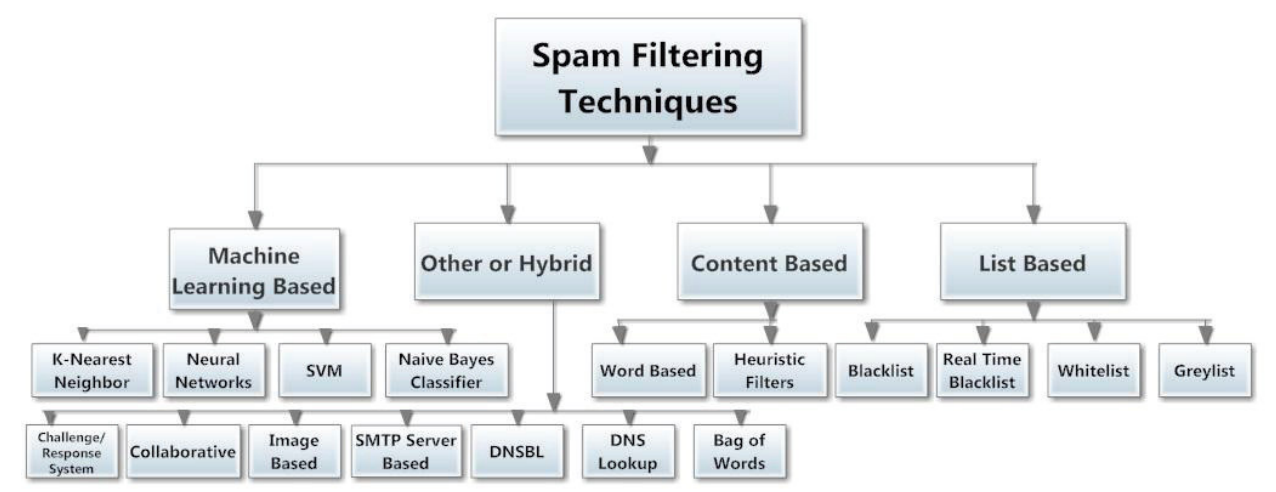
\includegraphics[width=\textwidth]{spam-filtering-techniques}
    \end{figure}
\end{frame}

\begin{frame}{Email Spam Filtering}
    \begin{columns}
        \column{0.25\textwidth}
            \begin{figure}
                \centering
                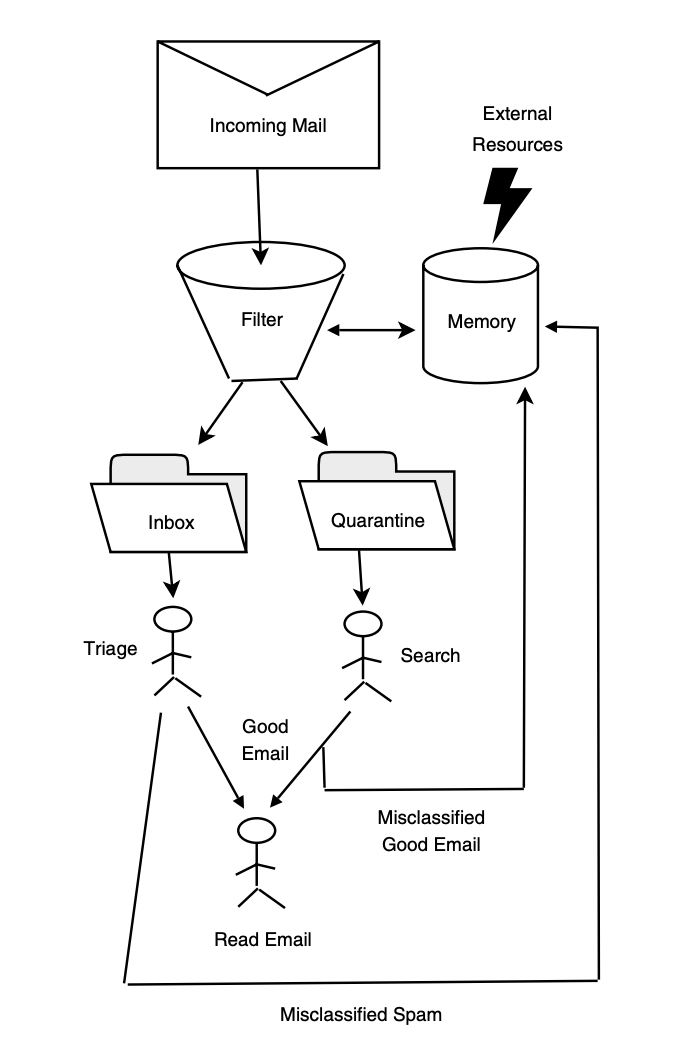
\includegraphics[width=\textwidth]{client-side-filter}
            \end{figure}
        \column{0.75\textwidth}
            \begin{figure}
                \centering
                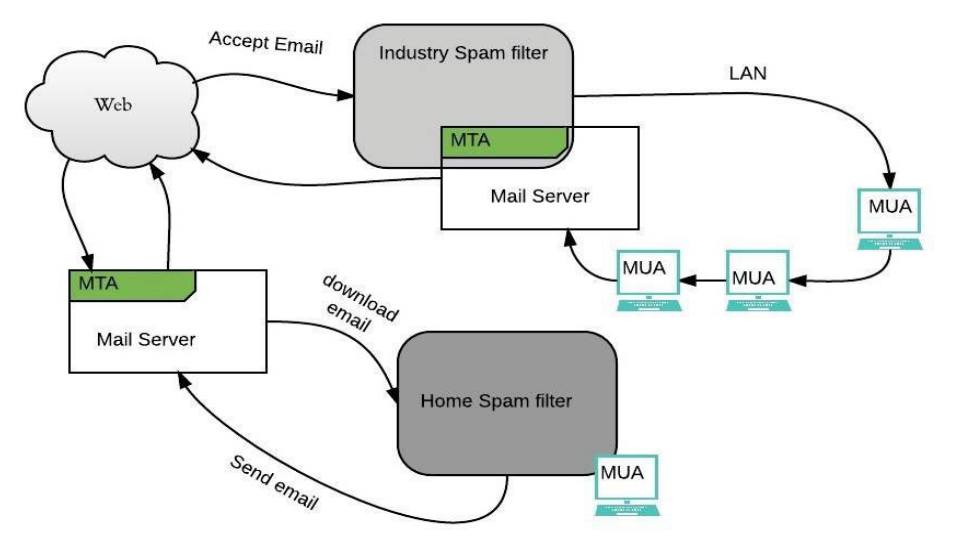
\includegraphics[width=\textwidth]{enterprise-side-filter}
            \end{figure}
            Client Side and Enterprise level Email spam filtering system
    \end{columns}
\end{frame}

\begin{frame}{Apache SpamAssassin}
    \begin{columns}
        \column{0.6\textwidth}
            \begin{itemize}
                \item Open-source tool that provides configurable spam filtering capabilities
                \item Scans the headers and message content, seeking the spam-related texts
                \item Uses a points based system
                \item When it finds particular characteristics in an email, it assigns a point value
                \item If the the email exceeds maximum point value, the email is flagged as spam
            \end{itemize}
        \column{0.4\textwidth}
            \begin{figure}
                \centering
                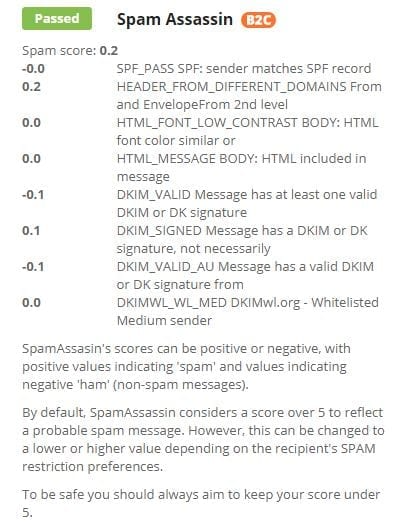
\includegraphics[width=\textwidth]{spam-assassin}
            \end{figure}
    \end{columns}
\end{frame}

\begin{frame}{SMTP AUTH}
    \begin{columns}
        \column{0.4\textwidth}
            \begin{figure}
                \centering
                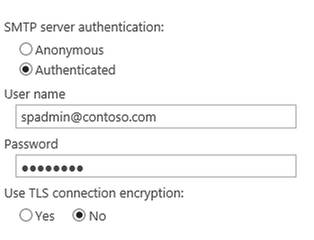
\includegraphics[width=\textwidth]{smtp-server-auth}
            \end{figure}
        \column{0.6\textwidth}
            Used from an MUA to an MTA.\\
            The MTA can then enforce restrictions on MAIL FROM and From:\\
            Useless MTA-MTA\\
            \begin{itemize}
                \item 100s of millions of MTAs send mail every day -- nobody wants to maintain passwords!
            \end{itemize}
    \end{columns}
\end{frame}

\begin{frame}{SPF - Sender Policy Framework}
    Used MTA-MTA
    When an MTA contacts another MTA, it is almost impossible to forge the sending MTA’s IP address.
    SPF lets a domain specify which IPs are OK to use a domain in MAIL FROM
    \begin{itemize}
        \item Users can’t see MAIL FROM
        \item SMTP is a relay system and senders don’t control the intermediate steps -- 5-10\% of valid mail will fail SPF due to automated forwarding
        \item SPF has all the features anybody wanted it to have
    \end{itemize}
\end{frame}

\begin{frame}{}
    \thispagestyle{empty}
    \begin{figure}
        \centering
        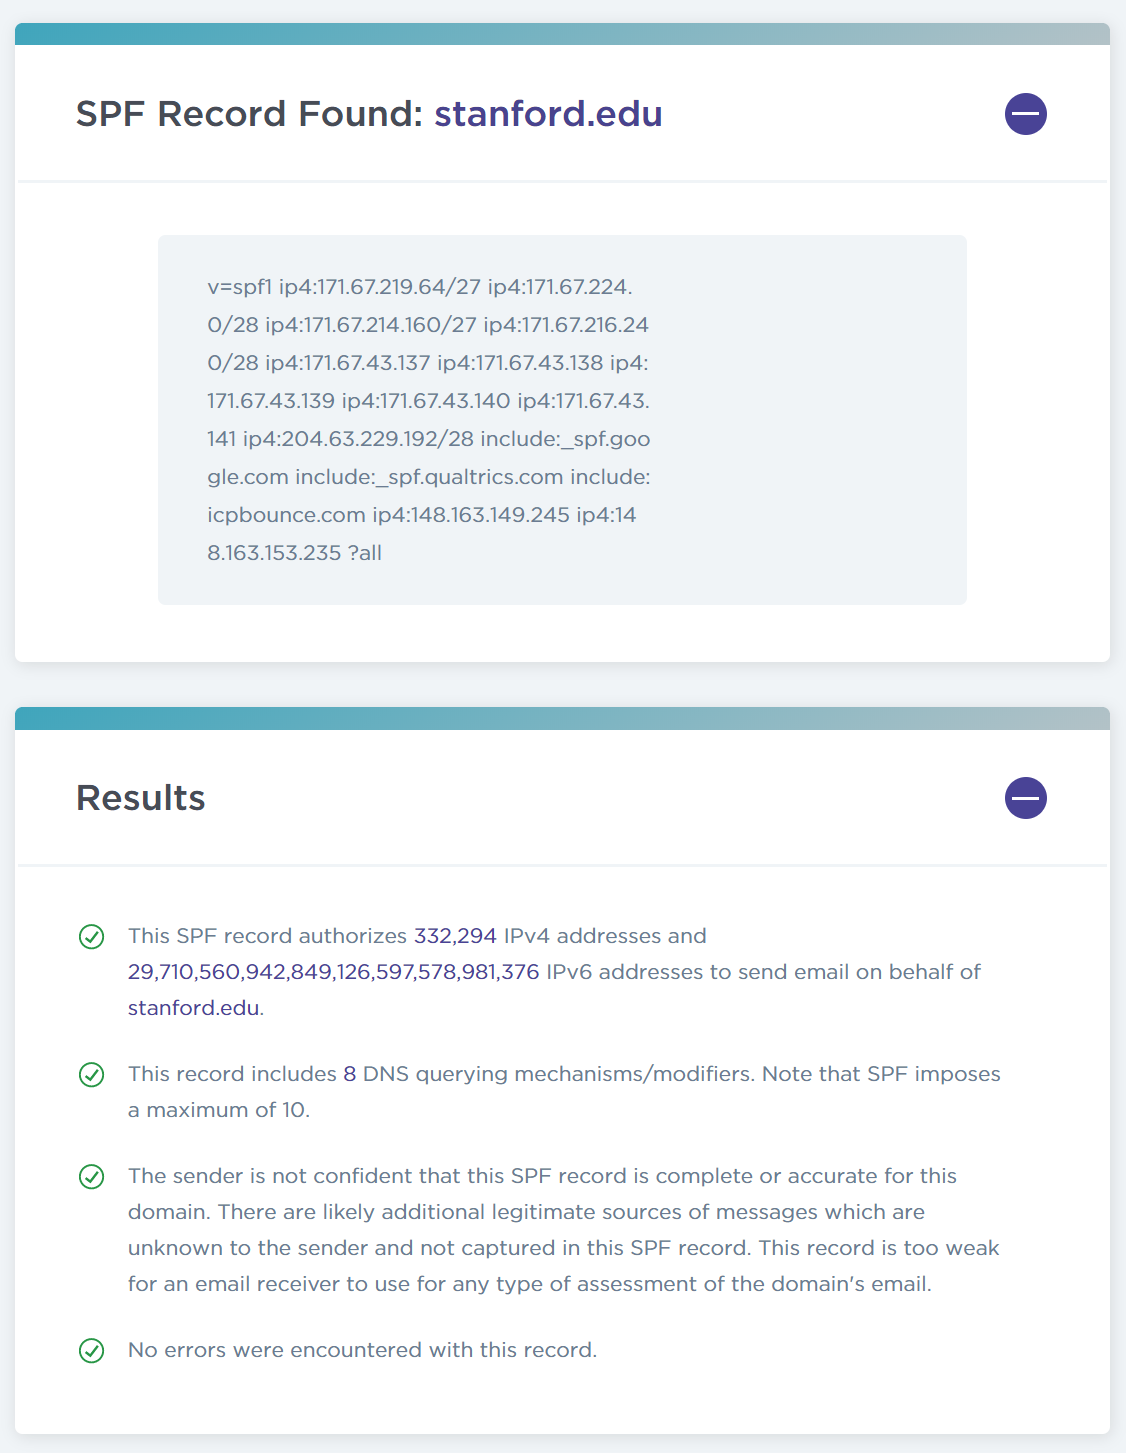
\includegraphics[height=\textheight]{spf-found}
    \end{figure}
    \url{https://www.agari.com/insights/tools/spf/?domain_name=stanford.edu}
\end{frame}

\begin{frame}{DKIM - Domain Keys Identified Mail}
    Used MTA-MTA\\
    Via public key cryptography, allows any handling MTA to assert
    \begin{itemize}
        \item that it at one point was able to read and modify the message
        \item what the signatures of specified headers and (optionally) the body were at that time
    \end{itemize}
    DKIM can survive autoforwarding but does not if the message is changed.\\
    DKIM signatures may or may not cover or relate to any user-visible header
\end{frame}

\begin{frame}{DMARC}
    An assertion which allows a domain to specify that there must be an affirmative pass for either SPF or DKIM that is aligned to the user-visible From:
    \begin{itemize}
        \item Affirmative pass = not failing is not good enough, must exist and pass
        \item Aligned = must be the domain the user sees in From: (although you can permit subdomains to pass)
    \end{itemize}
    Makes SPF and DKIM more useful by providing
    \begin{itemize}
        \item Reporting to domain owner
        \item User-visible semantics
        \item Added reliability of allowing either to pass
    \end{itemize}
\end{frame}

\begin{frame}{}
    \thispagestyle{empty}
    \begin{figure}
        \centering
        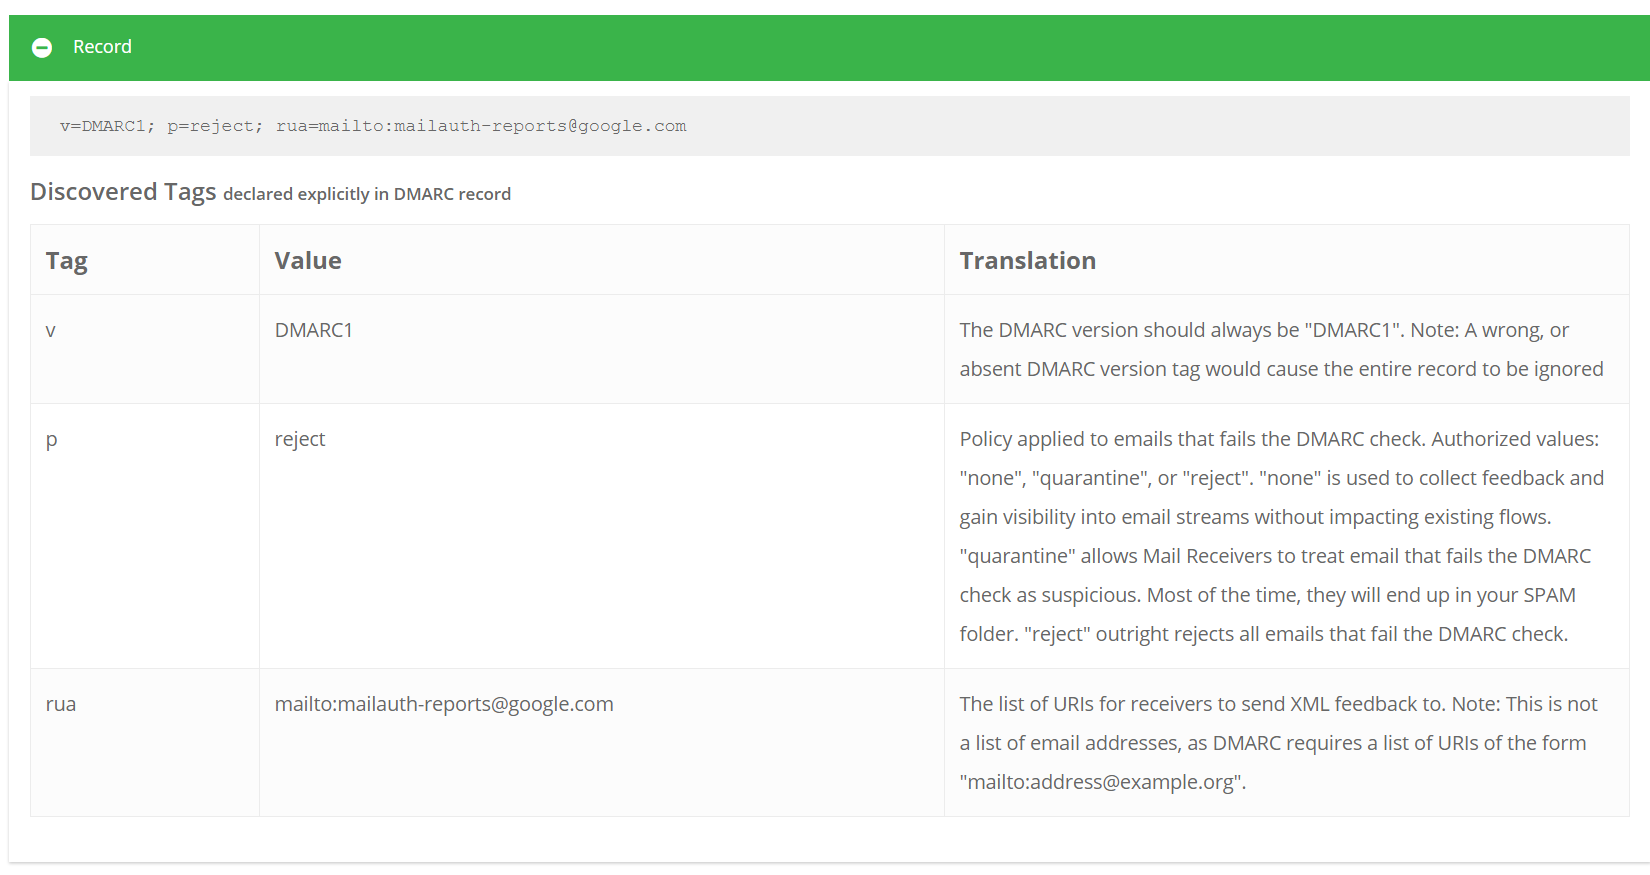
\includegraphics[width=\textwidth]{dmarc-discovered}
    \end{figure}
    \url{https://dmarcian.com/dmarc-inspector/}
\end{frame}

\begin{frame}{Fake Accounts}
    The robot army loves us all.
\end{frame}

\begin{frame}{But the Robot Army?}
    In order for you to buy accounts, someone either has to steal them or create them.\\
    Stealing them is illegal; making them is a violation of terms of service.\\
    So mostly people make them. By the millions. Every day.\\
    It’s more like a lot of robot mercenary groups, really. 
\end{frame}

\begin{frame}{Why Do They Love Anybody?}
    Because responding to or placing ads on dating sites is effective.\\
    The main scam is to claim to be a woman who wants to go out with a man but is scared and wants the man to verify a credit card first.\\
    Or maybe they just want you to meet them on a paid site.
\end{frame}

\begin{frame}{What Else Do They Do?}
    Everything that requires an email address.\\
    Obviously spam via email or on other platforms like Twitter or Instagram.\\
    Less obviously:
    \begin{itemize}
        \item Buy scarce things that can be resold
        \item Manipulate online polls that have some controls
        \item Be sold off individually for anonymous use
    \end{itemize}
\end{frame}

\begin{frame}{These Steps Interfere With the Economics of Spam} %THIS ONE SIMPLE TRICK WILL MAKE YOUR SPAM DISAPPEAR
    \begin{itemize}
        \item Spam is driven by making money
        \item Raise costs, lower revenues
        \item Take away the profit, and it will move
        \begin{itemize}
            \item Penalize affiliate marketing
            \item Target credit card processors who enable spammers to accept credit cards
            \item Infiltrate black market lists
            \item Stop counterfeit goods at the border
        \end{itemize}
    \end{itemize}
    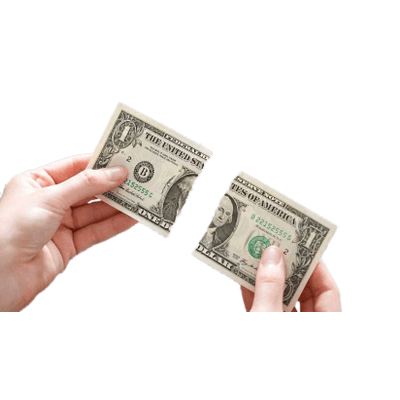
\includegraphics[width=0.39\textwidth, left]{torn-dollar}
\end{frame}

\begin{frame}{Target Scarce Resources}
    Words are in vast supply.\\
    Sending resources are readily available.\\
    People who want to buy your stuff are scarce.\\
    Money is not a scarce resource if you are willing to steal it.
\end{frame}

\begin{frame}{Where Is This Going?}
    \begin{itemize}
        \item Spammers and anti spammers are in an expensive meta stable state.
        \item Legal regimes constrained by borders.
        \item New tech capabilities => more abuse.
        \item Cryptocurrencies supercharge monetization
        \item New platforms repeat the pattern:
        \begin{itemize}
            \item Spam free nirvana
            \item Spam begins, things are unexpectedly awful!
            \item Battle commences, amid much misery.
            \item A stable state where users are exposed to a routine 20-30\% spam is reached and held with continued effort. 
        \end{itemize}
    \end{itemize}
\end{frame}

\backpage

\end{document}
